\chapter{Trajectory Generation}\label{app:trjgen}

\section{Differential Flatness}
% read references for interesting additions
% mention Hilbert and E. Cartan ?

Differential flat systems form a subclass of nonlinear control systems, where the flatness criterion can be seen roughly as an extension of Kalman's controllability (for linear systems) to nonlinear systems \cite{Fliess95}. These \emph{flat} systems are distinguished by the fact that trajectory generation can be performed explicitly, \emph{without} integration of the differential equation.

The nonlinear control system (or the system of underdetermined ordinary differential equations):

\begin{equation}
\dot{x} = f(x, u)
\label{ODE}
\end{equation}

where $x = (x_1,\ldots, x_n)$, $u = (u_1, \ldots, u_m)$ is said to be \emph{differentially flat}\footnote{This definition is taken from Scholarpedia: \url{www.scholarpedia.org/article/Differentially\_flat\_systems}} if and only if there exist $m$ independent functions $h = (h_1, \ldots, h_m) = h(x, u, u^{(1)}, u^{(2)}, \ldots, u^{(\alpha)})$ depending on $x$ and a finite number $\alpha$ of $u$'s derivatives such that, if we set 

\begin{equation}
y = h(x, u, u^{(1)}, \ldots, u^{(\alpha)}) \label{flat}
\end{equation}

the integral curves of \eqref{ODE} satisfy for some $\beta > 0$ :

\begin{eqnarray}
x = \Gamma(y, \ldots, y^{(\beta)}) \\
u = \Lambda(y, \ldots, y^{(\beta)})
\end{eqnarray}

Once the flat (also called linearizing) output given in \eqref{flat} is determined, the path planning problem becomes particularly easy: the reference trajectory as well as the corresponding feedforward (or open-loop) control can be expressed in terms of the flat output and a finite number of its derivatives \cite{Fliess95}.

The number of flat outputs is equal to the degree of freedom of the underdetermined ordinary differential equation \eqref{ODE}, i.e. the dimension of the control input $u$.
Unfortunately, deciding if a general nonlinear control system is flat is an open problem. Many mechanical systems are known to be flat \cite{Murray97nonlinearcontrol}.

A nice and easy example for a differential flat nonlinear system (all controllable linear systems are differential flat) is the vectored thrust aircraft model borrowed from \cite{Murray97nonlinearcontrol}:

\begin{equation}
\begin{aligned}
m \ddot{x}      & = F_{1}\cos{\theta} - F_{2}\sin{\theta} \\
m \ddot{y}      & = F_{1}\sin{\theta} - F_{2}\cos{\theta} - mg \\
J \ddot{\theta} & = r F_{1} 
\end{aligned}
\label{aircraftDynamics}
\end{equation}

where $m$ is the mass of the vehicle, $J$ is the moment of inertia, and $g$ the gravitational constant. Forces acting on the vehicle consist of $F_{1}$ acting perpendicular to the axis at a distance $r$ from the center of mass, and $F_{2}$, a force parallel to the axis of the vehicle, see Figure \ref{Aircraft} from \cite{AM08}.

\begin{figure}
\center
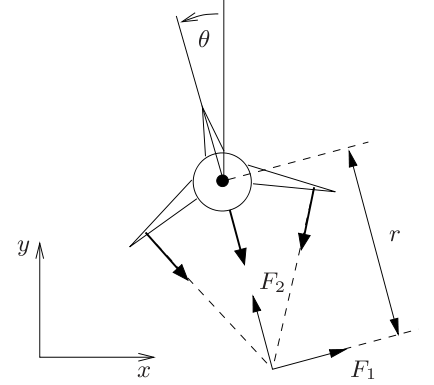
\includegraphics[scale=0.4]{aircraft.png}
\caption{Vectored thrust aircraft schematic}
\label{Aircraft}
\end{figure}

One set of flat outputs for this system is given by:

\begin{eqnarray}
z_{1} = x - (J/mr)\sin{\theta} \\
z_{2} = y + (J/mr)\cos{\theta} 
\end{eqnarray} 

Using system dynamics, the states and the control inputs $F_{1}, F_{2}$ can be found from $z_{1}$ and $z_{2}$ only. For example, $\theta$ can be found from:

\begin{equation}
\ddot{z}_{1} \cos{\theta} + (\ddot{z}_{2} + g) \sin{\theta} = 0
\end{equation}

except for the singularity $\ddot{z}_{1} = \ddot{z}_{2} + g = 0$.

See \cite{Fliess95} where the subject is introduced with \emph{dynamic feedback linearization} from a differential algebraic point of view. See \cite{Rathinam97} for a differential-geometric treatment of the subject.

\section{Splines Method}
\label{Splines}
% mention initialization, support points
% plan feasible quadrocopter trajectories (with respect to the constraints introduced) that track arbitrary user-defined shapes in the vertical plane.

In this section, we briefly summarize a method for generating feasible reference trajectories for differential flat systems under input constraints, following the spline based approach in ~\cite{ILC_Angela,Zhang}. In order to generate the desired trajectories and the nominal control inputs along those trajectories, first the geometry of the differential flat output trajectories are defined through splines. These high-order splines are generated from a few sample points and are assumed to be smooth enough to satisfy the system constraints. Next a motion profile defining the dynamics is generated in order to append time information to the purely geometric path. This profile, again based on splines, parametrizes the trajectory w.r.t time and has to be chosen smooth enough (i.e. of high enough order) to satisfy the feasibility constraints.

In the case of the quadrocopter dynamics, $y(t), z(t)$ are the differential flat outputs and $z(y)$ is the geometric path created using splines. $y(t)$ is then appended as a suitable motion profile to the geometric path. The feasibility constraints are as follows:

\begin{align}
f_{min} \leq f_i &\leq f_{max}, \label{thrust_constraints} \\
|\dot{f}| \leq &\dot{f}_{max}, \label{thrust_rate_constraints} \\
|\dot{\phi}| \leq &\dot{\phi}_{max}, \label{angular_acc_constraints} \\
|\ddot{\phi}| \leq &\ddot{\phi}_{max}, \label{angular_vel_constraints}
\end{align}

where $i \in{a,b,c,d}, $ are the indexes of the separate forces adding up to the total force $f_{\mathrm{coll}}$ in \eqref{yddot}, \eqref{zddot}. These constraints represent the thrust, rate of thrust, angular acceleration and angular velocity constraints respectively. Table \ref{table_parameters} contains all the constants and parameters we used in the simulations. In the learning phase, the constraints are modified to make more space for learning~\cite{ILC_Angela}. 

{\color{red}
\begin{table}[h!t]
% increase table row spacing, adjust to taste
\renewcommand{\arraystretch}{1.3}
\caption{Quadrocopter dynamical constraints}
\label{table_parameters}
\centering
\begin{tabular}{ccc}
\textbf{Constraints} & \textbf{Trajectory Generation} & \textbf{Learning} \\
\hline
$f_{min}$ & $0.4\ m/s^2$ & $0.25\ m/s^2$ \\
$f_{max}$ & $4.5\ m/s^2$ & $5.5\ m/s^2$ \\
$\dot{f}_{max}$ & $27\ m/s^3$ & $51\ m/s^3$ \\
$\dot{\phi}_{max}$ & $22\ rad/s$ & $25\ rad/s$ \\
$\ddot{\phi}_{max}$ & $150\ rad/s^2$ & $200\ rad/s^2$ \\
\end{tabular}
\end{table}
}

A quadrocopter motion profile generated for a wave-form trajectory is shown in Figure \ref{Lambda profile}. MATLAB \emph{fmincon} routine is used for finding optimal spline parameters. Note that this method has no guarantee of global optimality, and if care is not given, can get stuck in local optima.

\begin{figure}
\center
%\psfragfig[width=\columnwidth]{data/lambda}		
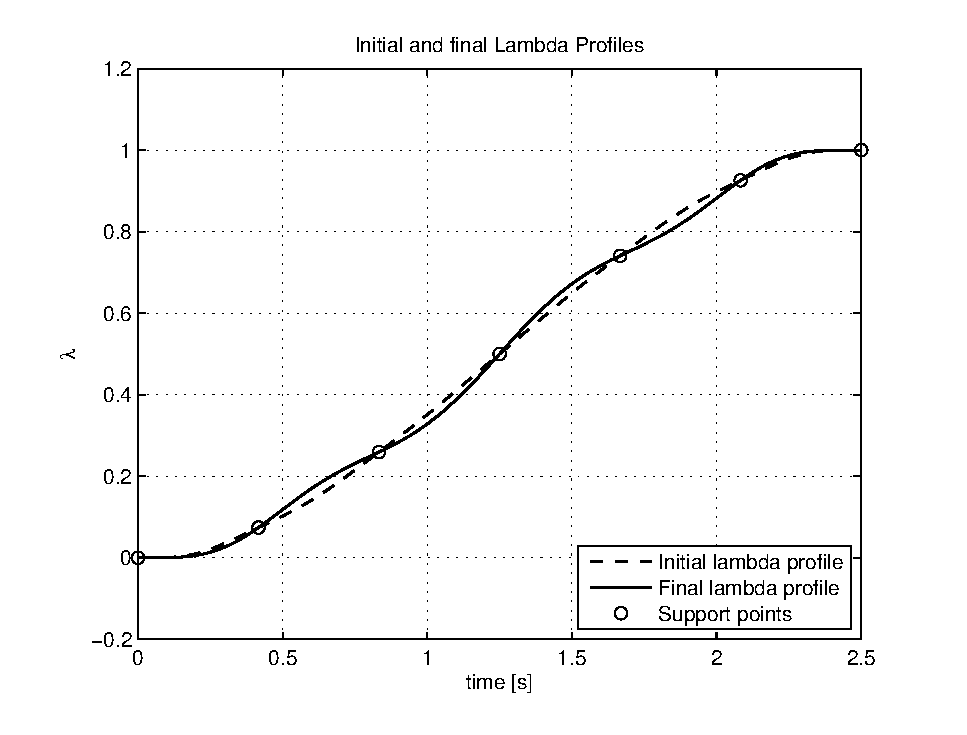
\includegraphics[scale=0.5]{lambda.eps}
\caption{Motion profile for a wave trajectory}
\label{Lambda profile}
\end{figure}

In Figure \ref{Quadrocopter} is shown a schematic drawing of a quadrocopter, taken from \cite{ILC_Angela}.

\begin{figure}
\center		
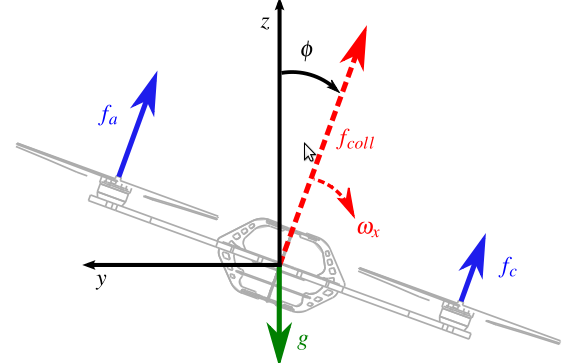
\includegraphics[scale=0.4]{quad.png}
\caption{A 2D schematic drawing of a quadrocopter}
\label{Quadrocopter}
\end{figure}
